% Chapter Template

\chapter{Desarrollo}

\label{Chapter4} % Change X to a consecutive number; for referencing this chapter elsewhere, use \ref{ChapterX}

Una vez presentado el contexto, los objetivos, así como las herramientas empleadas y los fundamentos teóricos, en este capítulo se detallará la solución software final desarrollada. Primero se presenta el diseño global utilizado y después se analizará en detalle el componente en cuestión realizado con una visión profunda del desarrollo por bloques y su funcionamiento.


%-----------------------------------
%	SECTION Diseño
%-----------------------------------
\section{Diseño}

El trabajo se basa principalmente en dos componentes; un componente de JDeRobot (\textbf{OpenniServer}) que funciona como driver del sensor y proporciona las imágenes obtenidas por éste y el componente realizado (\textbf{RealRTEstimator}) que se encargará, una vez recogidas las imágenes, de toda la lógica restante.

El objetivo del componente, como ya se ha comentado, consiste en analizar en tiempo real la posición y movimiento del sensor, por lo que el componente deberá dar una estimación en todo momento.

En la Figura~\ref{fig:diagram1} se puede apreciar el diagrama global de funcionamiento del componente desarrollado y su conexión con otros componentes para los diferentes datos de entrada.

\begin{figure}[th]
\centering
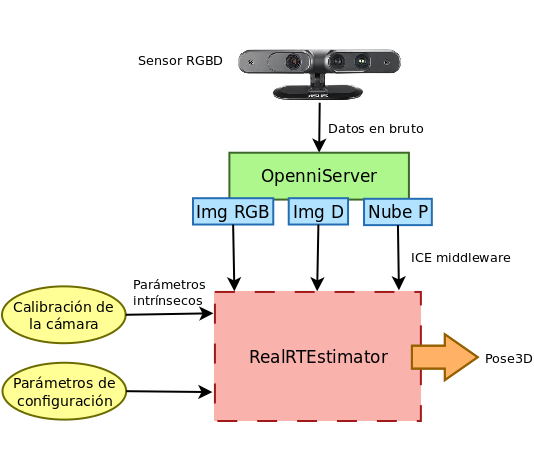
\includegraphics[scale=0.4]{Figures/diagram1.png}
\decoRule
\caption[Diagram1]{Esquema global de funcionamiento.}
\label{fig:diagram1}
\end{figure}

OpenniServer se encarga de preparar y enviar las imágenes del sensor. El componente recoge las imágenes a través de ICE y éste es el encargado de procesarlas. También recibe los datos de los parámetros intrínsecos de la cámara así como algunos parámetros de configuración, como pueden ser la activación/desactivación de la interfaz de usuario o algunos parámetros configurables de algunos de los algoritmos internos. A su salida entrega una matriz RT que describe la posición y orientación absolutas en ese preciso instante de tiempo. 

Respecto al funcionamiento interno del componente se puede ver a grandes rasgos el diagrama en la Figura~\ref{fig:diagram2}. Se observa el diseño implementado así como sus bloques funcionales:

\begin{figure}[!ht]
\centering
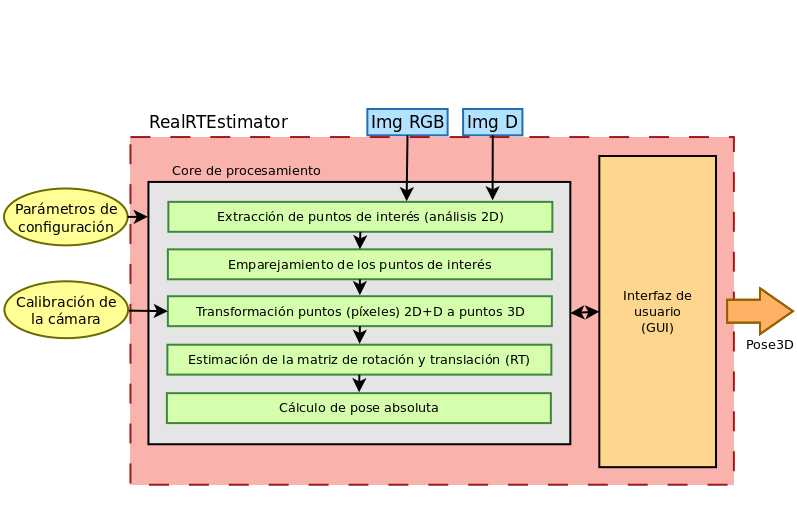
\includegraphics[scale=0.36]{Figures/diagram2.png}
\decoRule
\caption[Diagram2]{Diagrama del componente RealRTEstimator.}
\label{fig:diagram2}
\end{figure}

\begin{itemize}
\item Extración de puntos de interés (análisis 2D) del fotograma actual.

\item Emparejamientos de puntos de interés en t con respecto a los puntos extraídos en el instante anterior (t-1).

\item Transformación de puntos (píxeles) en 2D más imagen de profundidad a nube de puntos en 3D.

\item Cálculo de movimiento. Es decir, estimación de la matriz de rotación y translación (Matriz RT).

\item Calculo de pose 3D absoluta.

\end{itemize}

En las siguientes secciones desglosaremos el funcionamiento de estos diferentes bloques funcionales.

%-----------------------------------
%	SECTION Extracción de características de una imágen
%-----------------------------------
\section{Análisis 2D}

El primer bloque del componente RealRTEstimator es el de análisis 2D. A partir de dos imágenes; la imagen de color y la de profundidad, se procede a la extracción de puntos de interés.

\subsection{Puntos de interés}

El término puntos de interés o detección de características (\textit{Feature Detectio}n en inglés) hace referencia a la tarea de localizar en una imágen puntos relevantes o carácterísticos. Estos puntos suelen ser comunes y son fáciles de seguir de fotograma en fotograma.

Para entender cuales son estos puntos característicos podemos observar un ejemplo sencillo en la Figura~\ref{fig:feature_simple}. El cuadrado azul se encuentra en una área plana, y es difícil de seguir o encontrar. En cualquier lugar por donde se desplace parecerá que es el mismo. Para el cuadrado negro, que es un borde, igual para el desplazamiento lateral, sin embargo, para el desplazamiento vertical el punto ya cambia. Por último está el cuadrado rojo, que es una esquina. Para cualquier desplazamiento de esta figura, el punto ya es diferente, lo que significa que ese punto en la figura es único y por lo tanto vamos a poder identificarlo o seguirlo en diferentes imágenes. Así pues, las esquinas suelen ser candidatos idóneos para la detección puntos de carácterísticas en una imagen (en algunos casos las manchas también pueden ser consideradas buenas zonas).

\begin{figure}[!ht]
\centering
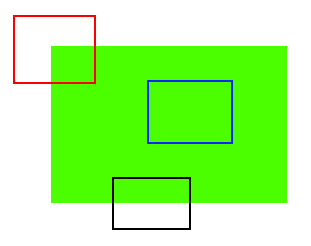
\includegraphics[scale=0.7]{Figures/feature_simple.png}
\decoRule
\caption[FeatureSimple]{Ejemplo sencillo de puntos característicos.}
\label{fig:feature_simple}
\end{figure}

Una vez entendido el concepto, el siguiente paso consiste, en averiguar cómo encontrar estos puntos de interés en una imagen real. Por ejemplo, una manera sencilla de hacerlo es buscar las regiones de las imágenes que contienen una gran variabilidad cuando son movidas (una pequeña distancia) hacia todas las regiones de los alrededores.

Existen multitud de implementaciones para calcular estas carácterísticas en las imágenes. Uno de los primeros intentos en encontrar estas esquinas fue hecho por Chris Harris y Mike Stephens \parencite{Reference8}. El método, llamado \textit{Harris Corner Detector} transforma la simple idea a una fórmula matemática (\ref{eqn:Harris}) que básicamente encuentra la diferencia en intensidad por un desplazamiento (u,v) en todas las direcciones.

\begin{equation}
E(u,v)\,=\,\sum_{x,y}w(x,y)\,\,[I(x\,+\, u,\, y\,+\, v)-I(x,y)]^{2}
\label{eqn:Harris}
\end{equation}

Donde \textit{w(x,y)} es una ventana rectangular o gaussiana e I(x,y) corresponde a la intensidad. Aplicando algunos cálculos matemáticos que no vamos a entrar en detalle podemos llegar a la ecuación (\ref{eqn:Harris}) básica que determina si una ventana contiene una esquina o no.

\[ R=det(m)-k(trace(M))^{2} \]
\begin{equation}
R=\lambda_{1}\lambda_{2}-k(\lambda_{1}+\lambda_{2})^{2}
\label{eqn:Harris2}
\end{equation}

$\lambda_{1}$ y $\lambda_{2}$ son los autovalores de la matriz M, que determinarán si una región es esquina, borde o zona plana.

\begin{itemize}
\item Cuando $|R|$ es pequeño, que sucede cuando $\lambda_{1}$ y $\lambda_{2}$ son pequeños, la región es plana.

\item Cuando $R < 0$, que sucede cuando $\lambda_{1} >> \lambda_{2}$ o viceversa, la región es un borde.

\item Cuando $R$ es grande, que sucede cuando $\lambda_{1}$ y $\lambda_{2}$ son grandes y más o menos iguales, la sección es una esquina.

\end{itemize}

Más tarde, J. Shi y C. Tomasi hicieron una pequeña modificación que obtuvo mejores resultados comparados con los obtenidos en el detector de Harris \parencite{Reference9}. El resultado del detector \textit{Shi-Tomasi Corner Detector} se puede ver en la ecuación~(\ref{eqn:Shi})

\begin{equation}
R=min(\lambda_{1},\lambda_{2})
\label{eqn:Shi}
\end{equation}

Si $R$ es mayor que un determinado umbral, o dicho de otro modo; solo cuando $\lambda_{1}$ o $\lambda_{2}$ se encuentran por encima de un valor mínimo $\lambda_{min}$, se considera que cierta región es esquina. En la Figura~\ref{fig:shi_detector} se puede observar el resultado de aplicar dicho algoritmo en una imagen.

\begin{figure}[ht]
\centering
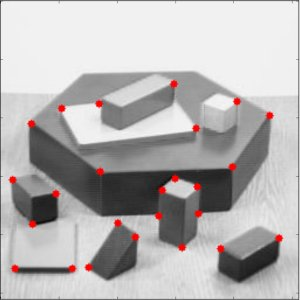
\includegraphics[scale=0.5]{Figures/shi-detector.jpg}
\decoRule
\caption[ShiDetector]{Resultado de encontrar las mejores 25 esquinas de la imagen con \textit{Shi-Tomasi Corner Detector}.}
\label{fig:shi_detector}
\end{figure}

Existen varias implementataciones para el cálculo de carácterísticas de una imagen. A parte de las mencionadas, las más conocidas pueden ser SIFT, SURF y FAST, proporcionadas todas por OpenCV.

\subsubsection{SIFT}

\subsubsection{SURF}

\subsubsection{FAST}

En el proyecto hemos hecho uso únicamente de SIFT y SIRF ya que permiten además de la detección de puntos de interés, el cálculo de descriptores que abordaremos en la siguiente sección.

%-----------------------------------
%	SECTION Emparejamiento (\textit{matching})
%-----------------------------------
\section{Emparejamiento (\textit{matching})}

%-----------------------------------
%	SUBSECTION Cálculo de movimiento
%-----------------------------------
\section{Cálculo de movimiento}

\subsection{Matriz RT}

%-----------------------------------
%	SECTION Interfaz gráfica
%-----------------------------------
\section{Interfaz gráfica}